%%%%%%%%%%%%%%%%%%%%%%%%%%%%%%%%%%%%%%%%%%%%%%
%                insertmeeting
% 1) Title (something creative & funny?)
% 2) Date (MM/DD/YYYY)
% 3) Location (ex. Hagerty High School)
% 4) People/Committees Present 
% 5) Picture 
% 6) Start Time & Stop Time (ex. 12:30AM to 4:30PM)
%%%%%%%%%%%%%%%%%%%%%%%%%%%%%%%%%%%%%%%%%%%%%%
\insertmeeting 
	{Umami Ultrasonics} 
	{02/08/22} 
	{Hagerty High School}
	{James, Jensen, Samantha, Anouska, Annika, Clayton, Falon, Nathan, Ritam}
	{Images/RobotPics/robot.jpg}
	{2:30 - 4:30}
	
\hhscommittee{Software}
\noindent\hfil\rule{\textwidth}{.4pt}\hfil
\subsubsection*{Goals}
\begin{itemize}
    \item Create an ultrasonic sensor that helps us maintain distance to the wall. 
    \item Write new vision for finding team elements.

\end{itemize} 

\noindent\hfil\rule{\textwidth}{.4pt}\hfil

\subsubsection*{Accomplishments}
A new problem that we experienced at the League championship was detecting the wall. One of the most difficult tasks for our robot was aligning to move perfectly through the gap between the barrier and wall. Upon further testing and inspection, it appeared that our distance sensor was not always aligned with the wall similar to the way it was during autonomous. This means that we could not directly apply the same method we used in autonomous to teleop. Our mentor then suggested using an ultrasonic sensor. By mounting the ultrasonic sensor on a servo, we could use a more reliable distance measrement that can also rotate to be facing flush with the wall at all times. The advantage of this would be better reliability during driving. This would greatly help our driver with cycles, parking, and scoring during teleop. 
The first step was having Nathan, one of our hardware specialists, design a mounting plate for the ultrasonic sensor. This would be put the ultrasonic sensor flush with the wall for the most accurate measurement. This was made quickly and cut on our school's Glowforge. 
The next step was in software. The first step was to find the heading of the robot using the built-in IMU (Inertial Measurement Unit). This was done through a quick call to the robot.gyro.getZHeading() method. After a simple conversion from degrees to servo position, we were able to send power to the servo. After that, the ultrasonic sensor was moving to align with the wall correctly. After testing a few values, the ultrasonic sensor was ready to be used. 

\begin{figure}[htp]
\centering
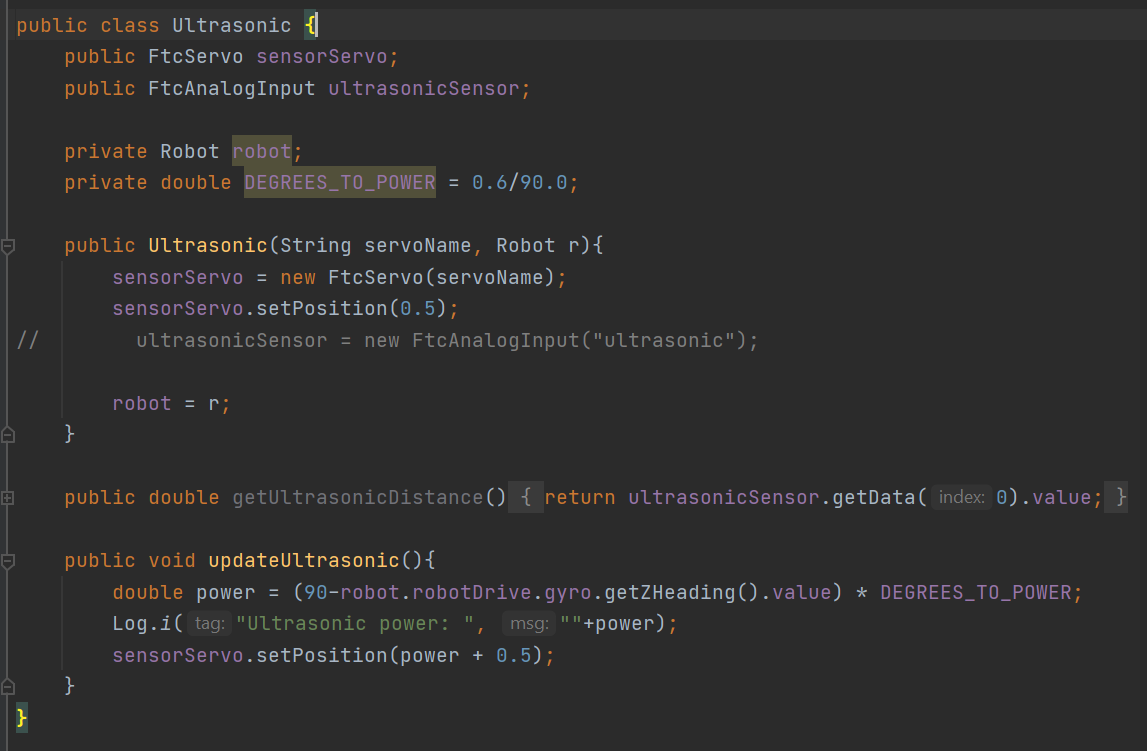
\includegraphics[width=0.95\textwidth, angle=0]{Meetings/February/02-08-22/02-08-22 1.PNG}
\caption{The code that will control the servo to move our ultrasonic sensor}
\label{fig:020822_1}
\end{figure}

\begin{figure}[htp]
\centering
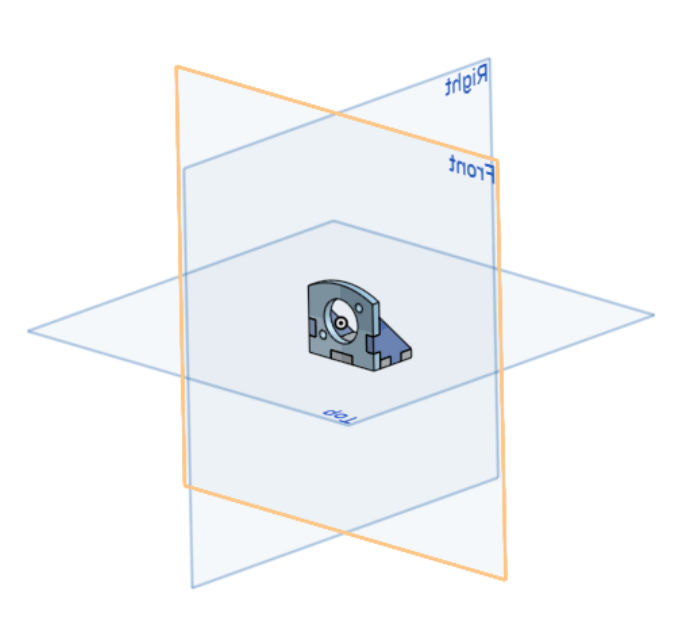
\includegraphics[width=0.95\textwidth, angle=0]{Meetings/February/02-08-22/02-08-22 2.PNG}
\caption{The CAD file for our ultrasonic sensor}
\label{fig:020822_2}
\end{figure}

\begin{figure}[htp]
\centering
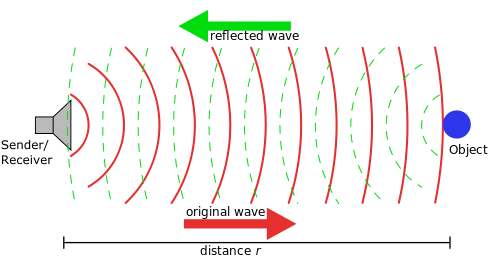
\includegraphics[width=0.95\textwidth, angle=0]{Meetings/February/02-08-22/02-08-22 3.PNG}
\caption{A diagram showing how we plan to use an ultrasonic sensor to determine the distance to the wall.}
\label{fig:020822_3}
\end{figure}



\hhscommittee{Software}
\noindent\hfil\rule{\textwidth}{.4pt}\hfil
\subsubsection*{Goals}
\begin{itemize}
    \item Create an ultrasonic sensor that helps us maintain distance to the wall. 

\end{itemize} 

\noindent\hfil\rule{\textwidth}{.4pt}\hfil

\subsubsection*{Accomplishments}
After seeing how the vision software we used at League Championships would find a green screen rather than our team element, we decided on making a vision software that would look for green in specified areas. Since the placement of our camera causes it to only see two out of the three barcodes, we draw two rectangles over each piece of tape for each side, for four in all. We continue to use the ranges of hue, saturation, and value of the team element. We look at the percent of green found in each rectangle when a team element is placed on the field. If the percent of green is above a certain threshold within one of the rectangles, then that determines the scoring level on the shipping hub. This gets rid of the chance of seeing any green in the background and mistaking it for our team element.

\whatsnext{
\begin{itemize}
    \item Implement ultrasonic sensor readings into the autonomous. 
    \item Work on autonomous
\end{itemize} 
}

